%This imports the file containing all of the configuration for the document
\documentclass [10pt]{article}
\oddsidemargin=0.0cm
\textwidth=16.5cm
\textheight=22.8cm
\topmargin=-1.0cm
\usepackage[utf8]{inputenc}
\usepackage{booktabs}
\usepackage{fancyhdr}
\usepackage{multicol}
\usepackage{mathtools}% Loads amsmath
\usepackage{lib/flowchart}
\pagestyle{fancy}
\fancyhf{}
\renewcommand{\headrulewidth}{1pt}
\usepackage{listings}

% the following is needed for syntax highlighting
\usepackage{color}
\usepackage{lib/arm} %arm keywords for syntax highlighting
\definecolor{dkgreen}{rgb}{0,0.6,0}
\definecolor{gray}{rgb}{0.5,0.5,0.5}
\definecolor{mauve}{rgb}{0.58,0,0.82}

\lstset{ %
language=[ARM]{Assembler},      % the language of the code
basicstyle=\scriptsize,         % the size of the fonts that are used for the code
numbers=left,                   % where to put the line-numbers
numberstyle=\tiny\color{gray},  % the style that is used for the line-numbers
stepnumber=1,                   % the step between two line-numbers. If it's 1, each line
% will be numbered
numbersep=5pt,                  % how far the line-numbers are from the code
backgroundcolor=\color{white},  % choose the background color. You must add \usepackage{color}
showspaces=false,               % show spaces adding particular underscores
showstringspaces=false,         % underline spaces within strings
showtabs=false,                 % show tabs within strings adding particular underscores
frame=single,                   % adds a frame around the code
rulecolor=\color{white},        % if not set, the frame-color may be changed on line-breaks within not-black text (e.g. commens (green here))
tabsize=2,                      % sets default tabsize to 2 spaces
captionpos=b,                   % sets the caption-position to bottom
breaklines=true,                % sets automatic line breaking
breakatwhitespace=false,        % sets if automatic breaks should only happen at whitespace
title=\lstname,                 % show the filename of files included with \lstinputlisting;
% also try caption instead of title
keywordstyle=\color{blue},          % keyword style
commentstyle=\color{gray},       % comment style
stringstyle=\color{mauve},         % string literal style
escapeinside={\%*}{*)},            % if you want to add a comment within your code
morekeywords={*,...}               % if you want to add more keywords to the set
}

\usepackage{float}

%header and Footer set up
\lhead{anandbal, asingh42}% Left Heading(Must by you and your partners UBIT name)
\rhead{Wee Dig Dug: Proposed Design}% Right Heading(Must be the title of the lab)
\rfoot{Page \thepage}% Right Footer - Page numbers
\lfoot{R1}% Left Footer
\title{Wee Dig Dug: Proposed Design}
\author{
	Anand Balakrishnan \\ \texttt{anandbal@buffalo.edu}
	\and
	Amrit Singh \\ \texttt{asingh42@buffalo.edu}
}
% Start the document
\begin{document}
  %%%%%%%%%%%%%%%%%%%%%%%

\maketitle
\tableofcontents\newpage


\section{Overall Flowsheet}

\begin{figure}[H]
	\centering
	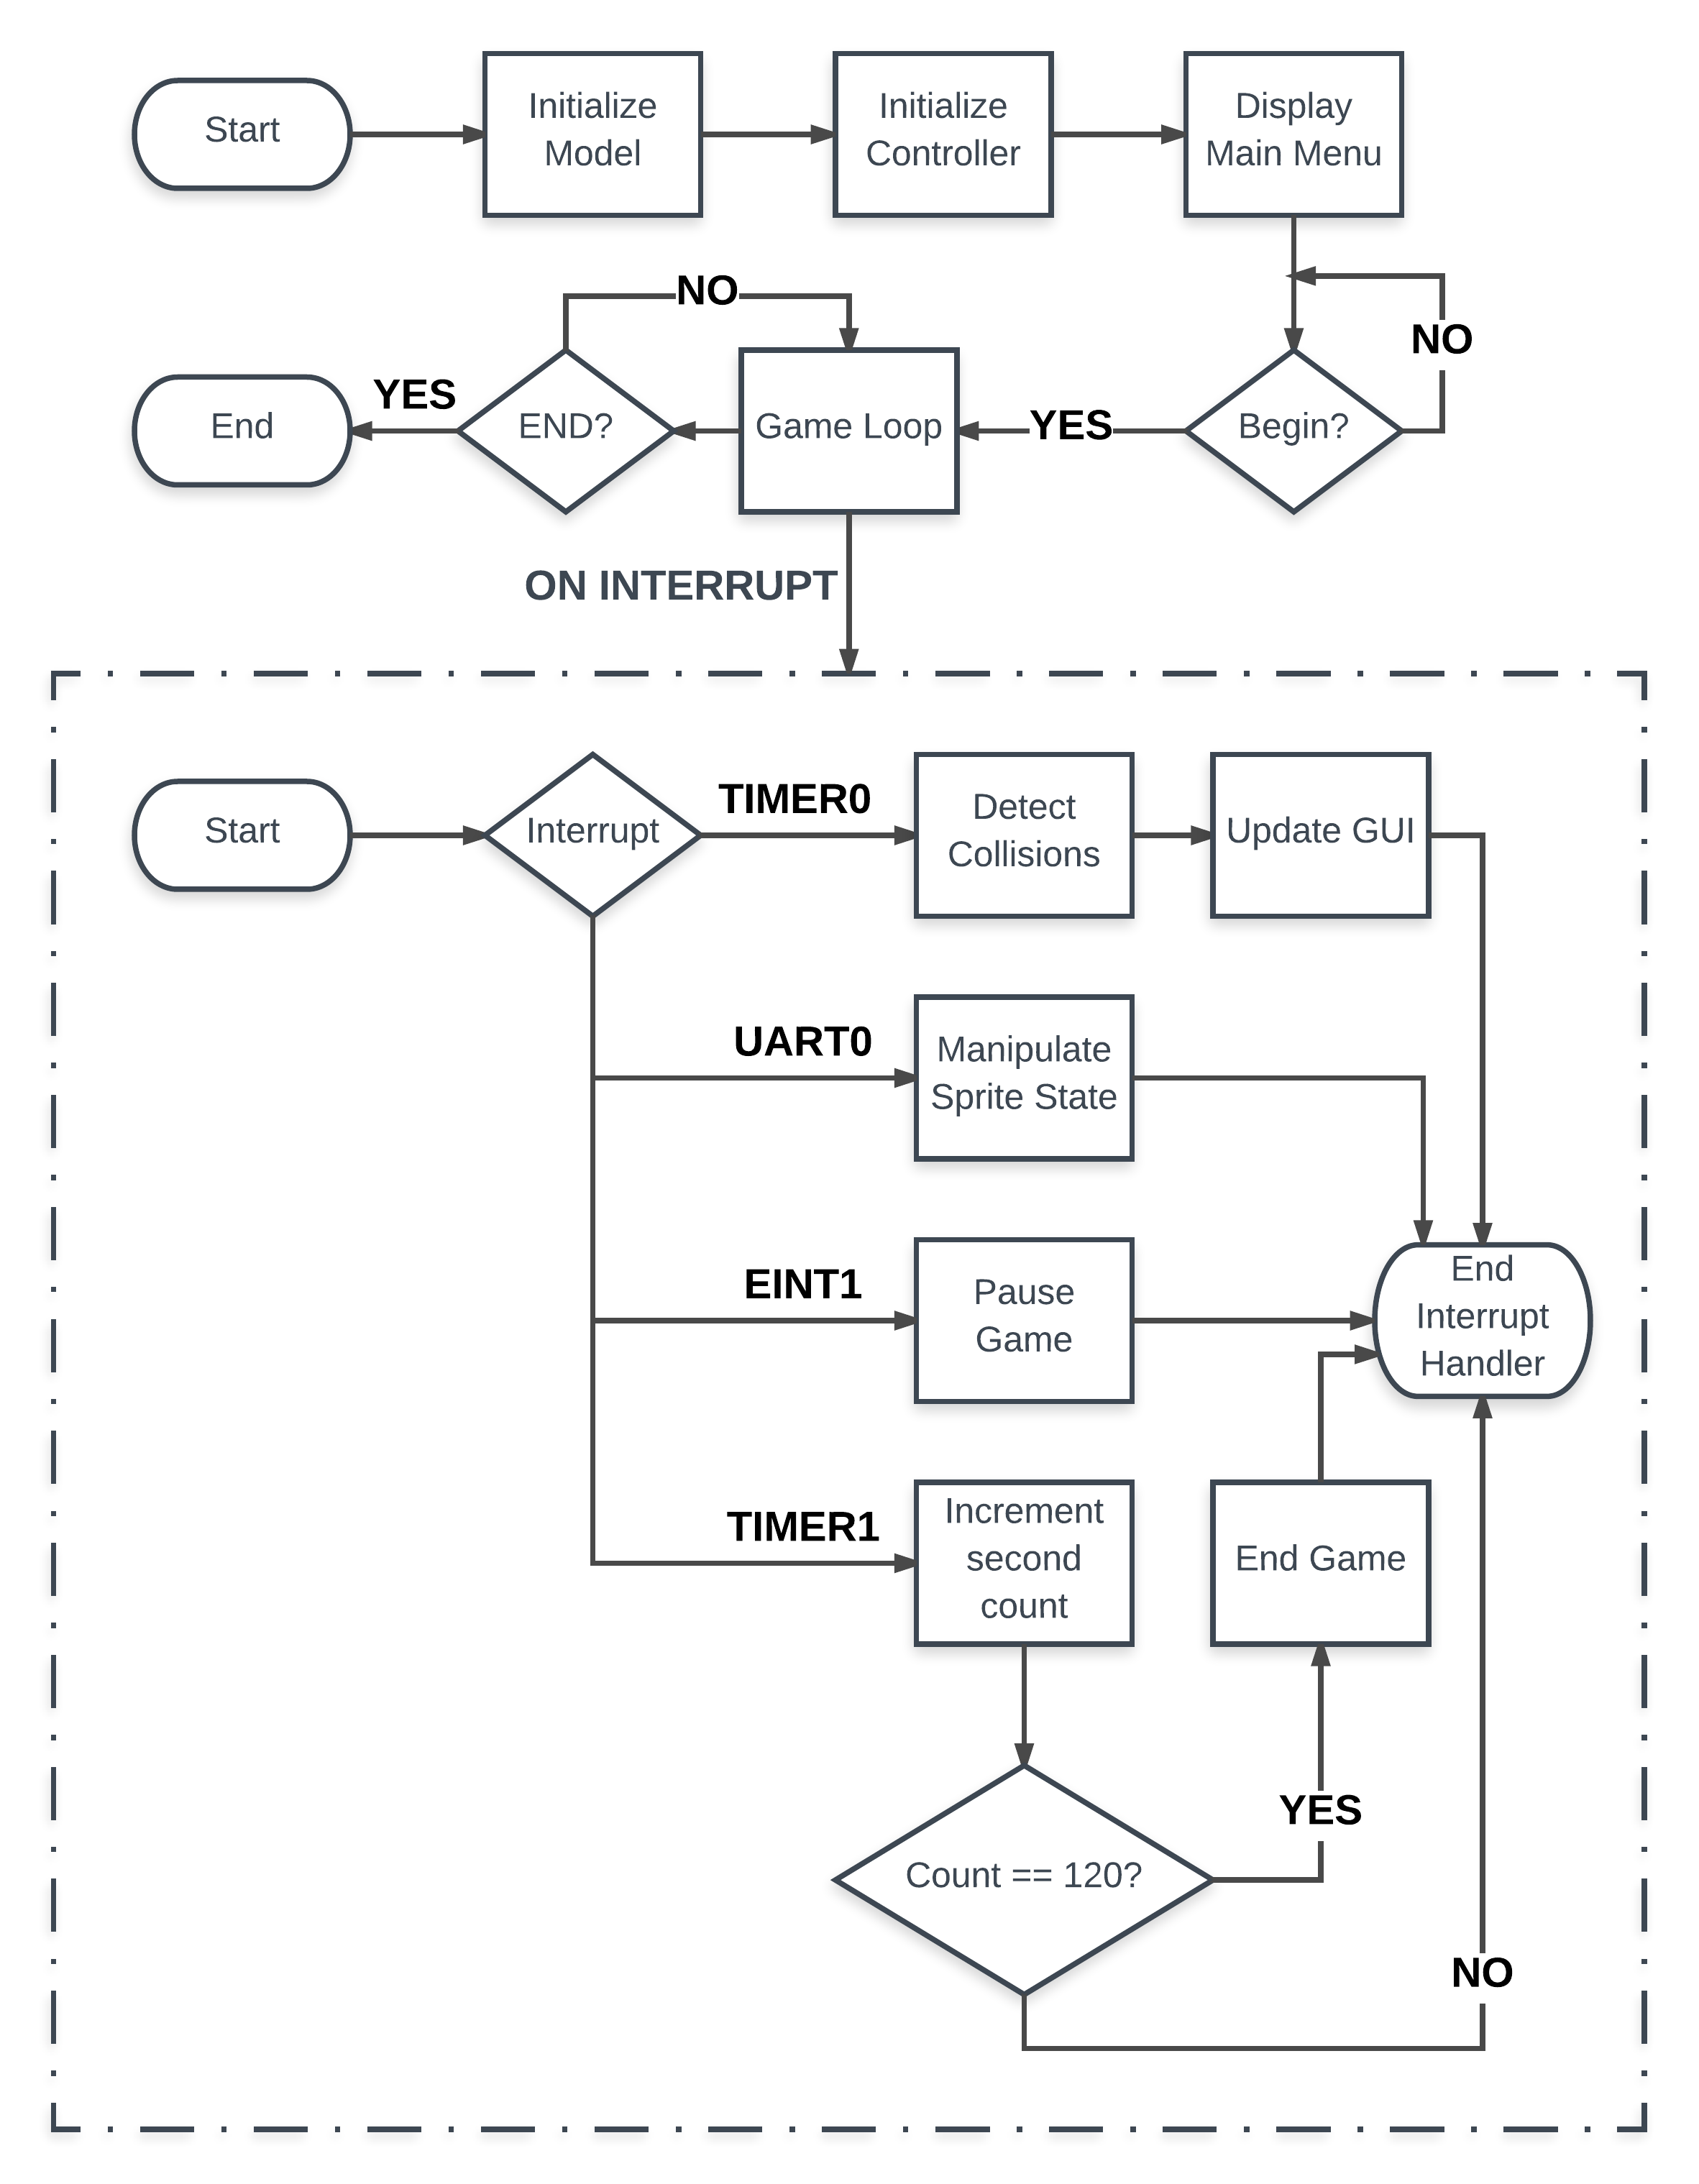
\includegraphics[width=0.8\linewidth]{flowsheets/overall.png}
	\caption{\label{fig:overall}Overall Flowsheet}
\end{figure}
\newpage

\section{Model: model.s}

Maintains the internal representation of the whole game.

\subsection{Uses}

The model will maintain the following information:

\begin{enumerate}
	\item Position and state of all sprites on board
	\item Position of all the sand using an array
	\item Score/Level
\end{enumerate}

\subsection{Subroutines}

The model contains subroutines that will:

\begin{itemize}
  \item Initialize model (board and sprites)
  \item Manipulate model
  \begin{itemize}
    \item Reset model
    \item Remove sprite
    \item Change sprite direction
    \item Remove sand and change score
  \end{itemize}
\end{itemize}

\subsection{Design}

The model consists of:

\begin{enumerate}
  \item The board: 40 X 64 array of "blocks".
  \begin{itemize}
    \item The board is a 40 X 64 byte array of blocks, each byte representing a boolean for sand, i.e, 1 = sand and 0 = no sand.
    \item The array is created by reserving 40*64 = 2560 bytes of space in static memory by using the SPACE or FILL directives.
    \item \textbf{NOTE:} The size of the array can be changed to make the game more space efficient. This can be addressed in later versions of the game
    \item \textbf{NOTE:} The size of the board can be changed also, as the final game should work regardless of size.
  \end{itemize}

  \item The sprites:
  \begin{itemize}
    \item Each type of sprite (Dug, his pump, Pookas and Fygars) maintains a position (the top left corner in GUI) and a state, (direction of movement, velocity, DEAD or not).
    \item The character sprites (Dug, the Pookas and the Fygars) are each of size 4 X 4 blocks (hence occupying 16 blocks).
    \item Dug's pump is a sprite of height 1 block and variable length. This sprite has an additional state variable to hold length. The length cannot exceed 4 blocks (**NOTE:** To be revised).
  \end{itemize}
\end{enumerate}

\section{GUI: gui.s}

The GUI reads the model and displays it.

\subsection{Function}

The GUI is responsible for the following:

\begin{itemize}
  \item Maintain the state of the screen, i.e., hold representation for Main Menu and Game
  \item Update itself as and when model is updated.
  \item Maintain a accurate representation of the model.
\end{itemize}

\subsection{Subroutines}

The GUI file will have subroutines that will:

\begin{itemize}
  \item Draw GUI
  \item Update GUI
\end{itemize}

\subsection{Design}

\begin{enumerate}

  \item Sand:
  \begin{itemize}
    \item Each block in the model represents one block of sand in the GUI.
    \item The sand is 4 X 4 "pixels" in the GUI.
  \end{itemize}
  
  \item Character Sprites:
  \begin{itemize}
    \item Each character sprite is 16 X 16 "pixels" in the GUI.
  \end{itemize}
  
  \item Draw/Update:
  \begin{itemize}
    \item The draw and update subroutines will print all variables in the model based on the pre-defined size of the sprites.
  \end{itemize}

\end{enumerate}

\section{Controller: controller.s}

The controller is the module that will control both, the GUI and the model.
It will mainly contain:

\begin{itemize}
  \item The interrupt handlers for user input and timer.
  \item Collision detection subroutine
  \item Update sprite positions subroutine
  \item Generate pump subroutine.
\end{itemize}

\subsection{Design:}

\begin{enumerate}
  \item For user input:
  \begin{itemize}
    \item Use FIQ Interrupts to handle user input/keystrokes, as implemented in Lab 6.
  \end{itemize}
  
  \item For game update:
  \begin{itemize}
    \item On timer interrupt, the controller has to perform collision detection and handling, and update position of sprites.
  \end{itemize}
\end{enumerate}


\subsubsection{Detecting collisions:}

\begin{enumerate}
  \item Read coordinate of each sprite in the model.
  \item For each sprite, do the following:
  \begin{itemize}
    \item For the Dug Sprite:
    \begin{enumerate}
      \item Sum up the byte values of all the blocks occupied by Dug on the Game board. Add to High Score.
      \item Set all blocks occupied by Dug to 0
      \item If blocks occupied by Dug overlap with that of either of the Pookas or Fygars, decrement Dug's life by 1, reset game.
      \item If collision with wall, do not update position.
    \end{enumerate}

    \item For the enemy sprites:
    \begin{enumerate}
      \item If collision with wall, set random direction.
    \end{enumerate}
  \end{itemize}
  
\end{enumerate}


\end{document}
